\documentclass[utf8]{ctexart}
\usepackage{graphicx}
\usepackage{amsmath, amssymb, amsthm}
\usepackage{geometry}
\usepackage{enumitem}
\usepackage{xcolor}
\usepackage{mdframed}
\usepackage{tikz}
\usetikzlibrary{graphs, positioning, arrows.meta}

\geometry{a4paper, margin=2.5cm}

% 定理环境
\newtheoremstyle{mystyle}
  {8pt}{8pt}{\kaishu}{0pt}{\bfseries}{}{1em}{}
\theoremstyle{mystyle}
\newtheorem{theorem}{定理}
\newtheorem{lemma}{引理}

% 好看的题目框
\newmdenv[
  linecolor=black!40,
  linewidth=1pt,
  backgroundcolor=gray!8,
  roundcorner=5pt,
  innertopmargin=8pt,
  innerbottommargin=8pt,
]{problembox}

\title{\textbf{离散数学2\quad 作业3}}
\date{\today}
\author{李子嘉 2024012325}
\begin{document}
\maketitle

\section*{题目1}

\begin{problembox}
证明：$G$ 和 $ \bar G$ 至少有一个是连通图。
\end{problembox}

\begin{proof}
不妨假设$G$是一个非连通图，我们需要证明$\bar G$是一个连通图。
任取$\bar G$中的任意两个顶点$u$和$v$，我们需要证明在$\bar G$中存在一条路径连接它们。
我们分两种情况讨论：
\begin{itemize}
    \item 如果$u$和$v$在$G$中属于不同的连通分量，那么在$\bar G$中，$u$和$v$之间存在一条边连接它们，直接满足要求。
    \item 如果$u$和$v$在$G$中属于同一个连通分量，由于$G$是非连通的，所以至少存在一个顶点$w$不在这个连通分量中。因此 $ u-w $ 和 $ v-w $ 都不是 $G$ 中的边，意味着它们是 $\bar G$ 中的边。所以通过顶点$w$，在$\bar G$中存在路径$u-w-v$连接$u$和$v$，满足要求。
\end{itemize}
综上所述，无论$u$和$v$在$G$中是否属于同一个连通分量，在$\bar G$中都存在一条路径连接它们，因此$\bar G$是一个连通图。
\end{proof}

\section*{题目2}
\begin{problembox}
证明：若连通图的最长道路不唯一，则它们必定相交。
\end{problembox}
\begin{proof}
我们采用反证法，假设$G$是一个连通图，$G$中存在两条最长道路$P$和$Q$，长度都为$l$，且$P$和$Q$不相交。

分别设$P$路径经过的顶点为$u_1, u_2, \ldots, u_{l}$，$Q$路径经过的顶点为$v_1, v_2, \ldots, v_{l}$。
由于$G$是连通的，存在一条路径$R$连接$u_i$和$v_j$，其中$1 \leq i, j \leq l$。

如果路径$R$与$P,Q$相交，而$P,Q$不相交，所以 $R$ 从 $u_i$ 出发必然在某个第一次离开 $P$ 的点，我们把它记作新的$u_i$，最终第一次到达 $Q$ 的某个点，我们把它记作新的$v_j$，
总而言之，我们可以调整$u_i,v_j$的选择，以确立新的路径$R$，使得$R$与$P,Q$都不相交。

设这条路径的长度为$d$，由于$P$和$Q$不相交，所以$d$至少为1。
随后，我们可以构造一条新的路径$R'$，从$P$的某个端点出发，沿着$P$走到$u_i$，然后沿着路径$R$走到$v_j$，最后沿着$Q$走到$Q$的某一个端点。
具体选择哪一个端点，我们根据分叉点$u_i$和$v_j$的位置来决定，以确保新路径在原路径$P,Q$中走过的长度最大。

我们可以这样计算新路径的长度：
\[
\text{长度}(R') = \max(i, l-i) + d + \max(j, l-j)
\]
由于$i$和$j$的取值范围是$1$到$l$，所以$\max(i, l-i) \geq \frac{l}{2}$，$\max(j, l-j) \geq \frac{l}{2}$，$d \geq 1$，因此：
\[
\text{长度}(R') \geq \frac{l}{2} + 1 + \frac{l}{2} = l + 1 > l
\]
这与$P$和$Q$是最长道路的假设矛盾。因此，我们的假设不成立，$P$和$Q$必定相交。
\end{proof}
\section*{题目3}
\begin{problembox}
在简单图中，证明：若 $ n \geq 4 $ 且 $ m \geq 2n -3 $，则 $ G $中含有带弦的回路。
\end{problembox}
\begin{proof}
我们采用反证法证明。假设$G$是一个简单图，满足$n \geq 4$且$m \geq 2n - 3$，但$G$中不含有带弦的回路。
我们将首先说明，\textbf{$G$的所有顶点中度数至少为3}，随后采用\textbf{极大路径法}推出矛盾。

我们取所有满足反证假设的图$G$中顶点数最少的一个图。假设$G$中存在一个顶点$v$，其度数小于3。\textbf{我们删除这一个顶点}。显然，\textbf{删除一个顶点不会使得图中出现带弦的回路}，因此删除后的图$ G' $也不含有带弦的回路。
删除一个顶点后，图中剩余的顶点数$n' = n-1$，边数$m' \geq m-3$（因为$v$的度数小于3）。由于$m \geq 2n - 3$，我们有：
\[
m' = m - 3 \geq 2n - 3 - 3 = 2(n-1) - 3 = 2n' - 3
\]
我们发现，删除一个度数小于3的顶点后，\textbf{剩余的图$ G' $仍然满足$m' \geq 2n' - 3$，并且不含有带弦的回路。}但是，$ n'=n-1 \geq 3 $，我们需要人工验证 $ n = 4$的情况，验证完毕后，我们可以断定$G$的顶点数$n \geq 5$，则$n' = n-1 \geq 4$，图$G'$ 满足了所有的条件。
接下来进行验证：

当$n=4$时，$m \geq 2n - 3 = 5$，一个有4个顶点的简单图最多只能有6条边，也就是完全图$K_4$。无论我们删去哪一条边，剩下的图都可以找到一个带弦的回路。
如下图所示，Case 1是删去外边框的一条边，Case 2是删去一条对角线。对于Case 1，v1-v3-v4-v2-v1是一个回路，v2-v3是它的弦；对于Case 2，v1-v2-v3-v4-v1是一个回路，v1-v3是它的弦。
\begin{center}
\textbf{Case 1: 删去外边框的一条边}

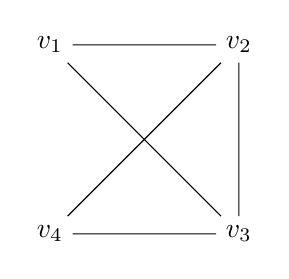
\begin{tikzpicture}[scale=1.2]
\node (v1) at (0,1) {$v_1$};
\node (v2) at (2,1) {$v_2$};
\node (v3) at (2,-1) {$v_3$};
\node (v4) at (0,-1) {$v_4$};

\draw (v1)--(v2);
\draw (v2)--(v3);
\draw (v3)--(v4);
% \draw (v4)--(v1); % 删除的边
\draw (v1)--(v3);
\draw (v2)--(v4);
\end{tikzpicture}

\bigskip

\textbf{Case 2: 删去一条对角线}

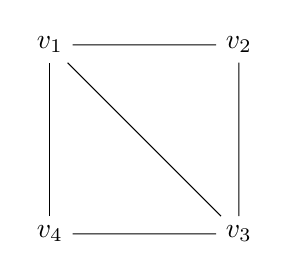
\begin{tikzpicture}[scale=1.2]
\node (v1) at (0,1) {$v_1$};
\node (v2) at (2,1) {$v_2$};
\node (v3) at (2,-1) {$v_3$};
\node (v4) at (0,-1) {$v_4$};

\draw (v1)--(v2);
\draw (v2)--(v3);
\draw (v3)--(v4);
\draw (v4)--(v1);
\draw (v1)--(v3);
% \draw (v2)--(v4); % 删除的边
\end{tikzpicture}
\end{center}
这样一来，我们验证了当$n=4$时，满足$m \geq 2n - 3$的图中必定存在带弦的回路，不满足反证假设。因此，我们可以断定$G$的顶点数$n \geq 5$，则$n' = n-1 \geq 4$，
图$G'$ 满足了所有的条件，并且顶点数更少，与我们选择的$G$是满足反证假设的图中顶点数最少的矛盾。因此，$G$中所有顶点的度数至少为3。

接下来，我们采用极大路径法。我们在$G$中选择一条最长路径$P$（不经过重复顶点），设$P$的长度为$k$，路径上的顶点依次为$u_1, u_2, \ldots, u_k$。
\textbf{由于$P$是最长路径，所以$P$的端点$u_1$和$u_k$不能有任何邻居不在$P$上，否则我们可以通过这个邻居构造出一条更长的路径，矛盾。}
根据$G$中所有顶点的度数至少为3这一条件，因此$P$的端点至少还有两个邻居。我们不妨假设$u_1$除$u_2$外的另外两个邻居是$u_{i}, u_{j}$，其中$2 < i < j \leq k$。

我们可以构造出一个回路$C$，路径为$u_1 - u_j - u_{j-1} - \ldots - u_i - u_{i-1} - \ldots - u_1$，即利用$u_1$与$u_j$的捷径跳过原最长路径的部分路段。
\textbf{然而，由于$u_1$与$u_i$也是邻居，所以$C$中存在一条弦$u_1-u_i$，因此$C$是一个带弦的回路，这与我们之前的假设矛盾。}因此，$G$中必定存在带弦的回路。
\end{proof}
\section*{题目4}
\begin{problembox}
  设$G$是不存在三角形的简单图，证明：
  \begin{enumerate}
    \item $\Sigma d^2(v_i) \leq mn$，其中$d(u)$表示顶点$u$的度数。
    \item $G$中边数$m \leq  \frac{n^2}{4} $。
  \end{enumerate}
\end{problembox}
\begin{proof}
我们首先证明第1部分。

由于$G$中不存在三角形，所以对于任意两个相邻的顶点$v_i$和$v_j$，它们的邻居集合是互不相交的。
具体而言，对于顶点$v_i$，有一个邻居是$v_j$；对于顶点$v_j$，有一个邻居是$v_i$。除此之外，
在其余的$n-2$个顶点集合$V \setminus \{v_i, v_j\}$中，每个顶点最多只能与$v_i$或$v_j$中的一个相邻，否则就会形成一个三角形。
我们可以据此得到以下不等式：
\[d(v_i) + d(v_j) \leq 1 + 1 + n - 2 = n\]
即，这两个顶点的度数之和，可以分成两部分计算：他们的直接连边各自贡献1；剩余的$n-2$个顶点最多只能与其中一个相邻，总和贡献不超过$n-2$。

我们对$G$中所有$m$条边$(v_i, v_j)$应用上述不等式，得到：
\[\sum_{(v_i, v_j) \in E} (d(v_i) + d(v_j)) \leq \sum_{(v_i, v_j) \in E} n = mn\]
由于每个顶点$v_i$的度数$d(v_i)$在上述求和中被计算了$d(v_i)$次（\textbf{每个顶点在所有边中出现的次数等于其度数}），我们可以将上式改写为：
\[\sum_{i=1}^{n} d^2(v_i) = \sum_{(v_i, v_j) \in E} (d(v_i) + d(v_j)) \leq mn\]
因此，我们证明了第1部分。
接下来，我们证明第2部分。
根据第1部分的结果，我们有：
\[\sum_{i=1}^{n} d^2(v_i) \leq mn\]
又因为$\sum_{i=1}^{n} d(v_i) = 2m$（\textbf{每条边贡献2个度数}），我们可以应用下面的不等式：
\[\left(\sum_{i=1}^{n} d(v_i)\right)^2 \leq n \sum_{i=1}^{n} d^2(v_i)\]
此式可以通过将$ b_1 = b_2 = \ldots = b_n = 1 $代入柯西-施瓦茨不等式得到，即平均值的平方不大于平方的平均值。
将$\sum_{i=1}^{n} d(v_i) = 2m$代入上式，得到：
\[(2m)^2 \leq n \cdot mn\]
\[4m^2 \leq n^2 m\]
即：
\[m \leq \frac{n^2}{4}\]
因此，我们证明了第2部分。

\end{proof}
\section*{题目5}
\begin{problembox}
证明：对于无向简单图$G$，若 $ |E(G)| \geq |V(G)| $，则$G$中存在一个回路。
\end{problembox}
\begin{proof}
我们给出两种证明方法：一种利用树的性质，另一种是删叶子节点的方法。

\textbf{法1：}我们用反证法，若 $G$ 中不存在回路，则 $G$ 为森林，其每个连通分量都是一棵树。
设 $G$ 有 $k$ 个连通分量 $G_1,G_2,\dots,G_k$，记
$|V(G_i)|=n_i$，$|E(G_i)|=m_i$。

由于每个 $G_i$ 是树，根据树的性质（每棵树的边数等于顶点数减一），我们有
\[
m_i = n_i - 1 \qquad (1\le i\le k).
\]

将各分量的边数相加，得到
\[
|E(G)|
= \sum_{i=1}^k m_i
= \sum_{i=1}^k (n_i-1)
= \left(\sum_{i=1}^k n_i\right) - k
= |V(G)| - k.
\]

由于 $k \ge 1$，于是
\[
|E(G)| \le |V(G)| - 1.
\]

与假设 $|E(G)| \ge |V(G)|$，矛盾，因此 $G$ 中必存在回路。

\textbf{法2：}我们同样用反证法，假设 $G$ 中不存在回路，且 $|E(G)| \geq |V(G)|$。
我们知道，\textbf{无回路图必定存在一个度数不超过1的顶点}（叶子节点）。否则，若所有顶点的度都至少为 $2$，则从任意顶点出发都能沿边不断前进（因为每个顶点至少有两条边，一进一出），
而顶点数是有限的，必然会回到已经访问过的顶点，从而形成回路，与假设矛盾。

我们每次都选择删除一个度数为1的顶点（叶子节点），并把其唯一的边也删除。每删除一个顶点，我们同时删除一条边，因此在删除 $k$ 个叶子节点后，图中剩余的顶点数为 $|V(G)| - k$，边数为 $|E(G)| - k$。
\textbf{由于删除顶点不会增加回路的数量，因此删除后的图仍然不存在回路。}我们可以反复迭代删除，直到所有顶点度数都为0，这意味着我们删除了所有$|V(G)|$条边，也删除了$|E(G)|$个顶点。
由于最后至少会留下一个度数为0的顶点，我们必须在删除完所有顶点之前就删除了所有边，即 $|E(G)| < |V(G)|$，与假设 $|E(G)| \geq |V(G)|$ 矛盾。因此，$G$ 中必存在回路。
\end{proof}
\end{document}